\scanpage{52}
\mspage{51}
qui est un comorphisme d'ateliers

2) 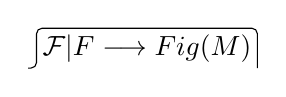
\begin{tikzpicture}[baseline=(v.base)]\node[inner sep=2pt] (v) {$\unsure{\mathcal F|\mathscr F}\longrightarrow\operatorname{Fig}(M)$};\draw[rounded corners=2pt] ([xshift=-3pt]v.south west)--(v.south west)--(v.north west)--(v.north east)--(v.south east);\end{tikzpicture} est un comorphisme d'ateliers injectif, satisfaisant la condition \inserted{de bijectivité} (1.54). En le composant avec des comorphismes \unsure{Fig}
\[
\operatorname{Fig}(M)\unsure{-|\to}\operatorname{Fil}(L)
\]
\unsure{déduit|induit|évident} comme dans $1^\circ$ \unsure{des|de} $L\unsure{\hookrightarrow|\subset}M$, on trouve des comorphismes
\[
\mathcal F-\operatorname{Fig}(L)
\]
\deleted{\unsure{l'un et}}\inserted{comme} l'autre, \inserted{il} satisfont la condition suppl. \inserted{\deleted{\unsure{de}} de bijectivité} (1.54), si cette fois on suppose \uline{At} 8 ; et sans \uline{que} $f$ soit \unsure{néc.} injectif.

\uline{Définition} On dit qu'un comorphisme $f:\mathcal F'\to\mathcal F$ d'ateliers est un co\uline{plongement}, si

\deleted{a) $f$ est injectif}

\deleted{\unsure{b)}}a) l'image $f(\mathcal F')$ est un sous-atelier de $\mathcal F$ \inserted{(p. \unsure{43|47})}
\par b) $f$ induit un iso. $\mathcal F'\unsure{\stackrel{\sim}{-}|\xrightarrow{\sim}}f(\mathcal F')$.
% slanted
\margin{Comparer avec perplexité marginale bas page 47}

\deleted{\unsure{Cel}} Les conditions \unsure{a)} b) équivalent \unsure{(}compte tenu de a) à : \par a') $\forall\,F'\in\mathcal F'$, \inserted{posant $F=f(F')$} l'application
\begingroup\csname tagsleft@true\endcsname
\[
\operatorname{Sousfig}(F')\longrightarrow\operatorname{Sousfig}(F)\qquad G'\unsure{\mapsto|-} f(G')\tag*{$(*)$}
\]
\endgroup
est bijective, \inserted{ou seulement} \deleted{\unsure{i.e.}}\deleted{\unsure{(comme}} elle est déjà injective par l'inj. de $f$, qui résulte de b) la surjectivité :
\[
\forall\,G\leq F,\ \exists\,G'\leq F'\quad\text{telle que}\quad G^{\unsure{*}}=f(G').
\]

b') $\forall\, F',\deleted{\unsure{F}}G'\deleted{\unsure{F|G}},\in \unsure{F'|\mathcal F'}$, on a
\[
f(G')\ll f(F')\Longrightarrow G'\ll F'
\]
% slanted
\margin{\uline{NB} Si $f$ est injective, alors $\mathrm{a}')\Rightarrow\mathrm{a})$, cf plus bas.}
